\section{Introduction}
In many data science problems, data are available through different views. In general, views represent different measurement modalities such as audio and video, or the same text can be available in different languages. Our main interest here is neuroimaging where recordings are made from several subjects. In particular, it is of interest to find common patterns or responses that are shared between subjects when they receive the same stimulation or perform the same cognitive task \citep{chen2015reduced,richard2020modeling}. 

A popular line of work to perform such shared response modeling is given by group independent component analysis (ICA) methods. The fastest methods~\cite{calhoun2001method, varoquaux2009canica} are among the most popular, yet they are not grounded on principled probabilistic models for the multiview setting. 
%
More principled approaches exist~\cite{richard2020modeling, guo2008unified}, however they do not model subject specific-deviations from the shared response; the magnitude of the response may differ across subjects \cite{penny2007random}, as does any noise due to heart beats, respiratory artefacts or head movement~\cite{liu2016noise}.
%
More importantly, most GroupICA methods are typically unable to separate Gaussian components.

Independent vector analysis (IVA)~\cite{lee2008independent, anderson2011joint} suggests a powerful framework, where components are independent within views but each component of a given view can depend on the corresponding component in other views. 
%
However, the two most common implementations (IVA-L~\cite{lee2008independent} and IVA-G~\cite{anderson2011joint}) only estimate view-specific components, and do not model or extract a shared response. 
%\bt{What versions of IVA ? need to be more precise}
%
They are thus not well-suited for modelling the dependencies between views in functional brain imaging, as we will argue in detail below. On the other hand, the shared response model~\cite{chen2015reduced} is a popular approach to perform shared response modeling, yet it imposes orthogonality constrains that are too restrictive and not biologically plausible.

In this work we introduce Shared ICA (ShICA), where each dataset is modeled as a linear transform of shared independent components contaminated by additive Gaussian noise. ShICA allows for principled extraction of the shared components (or responses) in addition to view-specific components. 
%
Since it incorporates a statistically sound noise model, it enables optimal inference (minimum mean squared error, MMSE) of the shared responses.
%, as well as the parameters modelling individual differences.
% \ag{last sentence can be improved}

The paper is organized as follows.
We first analyse the theoretical properties of the ShICA model, before providing powerful inference algorithms.
First, we exhibit necessary and sufficient conditions for ShICA to be identifiable (previous work only shows local identifiability~\cite{anderson2014independent}), in the presence of Gaussian or non-Gaussian components. 
%
We then introduce an algorithm called ShICA-J that uses Multiset CCA to fit the model when all the components are assumed to be Gaussian. We exhibit necessary and sufficient conditions for Multiset CCA to be able to fit the model (previous work only gives sufficient conditions~\cite{li2009joint}) and provide examples on which ShICA-J can recover the mixing matrices, while Multiset CCA cannot. 
%
We next point out a practical problem, namely that even a small sampling noise can lead to large rotations of unmixing matrices when Multiset CCA is used. To address this issue and recover the correct unmixing matrices, we propose to apply joint diagonalization to the result of Multiset CCA.
%
We further introduce ShICA-ML, a maximum likelihood estimator of ShICA that models non-Gaussian components using a Gaussian mixture model. 
%
While ShICA-ML yields more accurate components, ShICA-J is significantly faster and offers a great initialization to ShICA-ML.
Experiments on fMRI and MEG data demonstrate that the ensuing method outperforms existing GroupICA and IVA methods.


\section{Shared ICA (ShICA): an identifiable multi-view model}
\paragraph{Notations} We write vectors in bold letter $\vb$ and scalars in lower case $a$. Upper case letters $M$ are used to denote
matrices. We denote $|W|$ the absolute value of the determinant of $W$. $\xb \sim \Ncal(\mub, \Sigma)$ means that $\xb \in \mathbb{R}^k$ follows
a multivariate normal distribution of mean $\mub \in \mathbb{R}^k$ and
covariance $\Sigma \in \mathbb{R}^{k \times k}$. The $j, j$ entry of a diagonal matrix $\Sigma_i$ is denoted $\Sigma_{ij}$, the $j$ entry of $\yb_i$ is denoted $y_{ij}$. Lastly, $\delta$ is the Kronecker delta.

\paragraph{Model Definition} In the following, $\xb_1, \dots ,\xb_m \in \bbR^p$ denote the $m$ observed random vectors obtained from the $m$ different views. We posit the following generative model, called Shared ICA (ShICA): for $i= 1\dots m$
\begin{equation}
  \label{eq:model}
   \xb_i = A_i(\sbb + \nb_i)
\end{equation}
where $\sbb \in \mathbb{R}^{p}$ contains the latent variables giving the \emph{shared components}, $A_1,\dots, A_m\in\bbR^{p\times p}$ are invertible mixing matrices, and $\nb_i \in
\mathbb{R}^{p}$ are \emph{individual noises}. The individual noises model both the deviations of a view  from the mean ---i.e.\ individual differences--- and measurement noise. Importantly, we explicitly model both the shared components and the individual differences in a probabilistic framework to enable an optimal inference of the parameters and the responses.

We assume that the shared components are statistically independent, and that the individual noises are Gaussian and independent from the shared components:
$p(\sbb) = \prod_{j=1}^p p(s_j)$ and $\nb_i \sim\mathcal{N}(0, \Sigma_i)$, where the matrices $\Sigma_i$ are assumed diagonal and positive. Without loss of generality, components are assumed to have unit variance $\bbE[\sbb \sbb^{\top}] = I_p$. We further assume that there are at least 3 views: $m \geq 3$. 

In contrast to almost all existing works, we assume that some components (possibly all of them) may be Gaussian, and denote $\mathcal{G}$ the set of Gaussian components: $\sbb_j \sim \mathcal{N}(0, 1)$ for $j \in \mathcal{G}$. The other components are non-Gaussian: for $j\notin \mathcal{G}$, $\sbb_j$ is non-Gaussian.
%We denote $g$ the number of Gaussian components.


\paragraph{Identifiability} The parameters of the model are $\Theta = (A_1, \dots, A_m, \Sigma_1, \dots, \Sigma_m)$. We are interested in the identifiability of this model: given observations $\xb_1,\dots, \xb_m$ generated with parameters $\Theta$, are there some other $\Theta'$ that can generate the same observations?
Let us consider the following assumption that requires that the individual noises for Gaussian components are sufficiently diverse:
%
\begin{assumption}[Noise diversity in Gaussian components]
\label{ass:diversity}
For all $j, j' \in \mathcal{G}, j \neq j'$, the sequences $(\Sigma_{ij})_{i=1 \dots m}$ and $(\Sigma_{ij'})_{i=1 \dots m}$ are different where $\Sigma_{ij}$ is the $j, j$ entry of $\Sigma_i$
\end{assumption}

It is readily seen that there is one trivial set of indeterminacies in the problem: if $P \in \mathbb{R}^{p \times p}$ is a sign and permutation matrix the parameters $(A_1 P, \dots, A_m P, P^{\top}\Sigma_1 P, \dots, P^{\top} \Sigma_m P)$ also generate $\xb_1,\dots, \xb_m$. The following theorem shows that under the above assumption, these are the only indeterminacies of the problem.

\begin{theorem}[Identifiability]
\label{thm:identif}
We suppose Assumption~\ref{ass:diversity}. We let $\Theta'=(A_1', \dots, A_m', \Sigma_1', \dots,\Sigma_m')$ another set of parameters, and assume that they also generate $\xb_1,\dots, \xb_m$. Then, there exists a sign and permutation matrix $P$ such that for all $i$, $A_i'=A_iP$, and $\Sigma_i'= P^{\top} \Sigma_i P$.
\end{theorem}
The proof is in Appendix~\ref{proof:identif}. Identifiability in the Gaussian case is a consequence of the identifiability results in~\cite{via2011joint} and in the general case, local identifiability results can be derived from the work of ~\cite{anderson2014independent}. 
%
However local identifiability only shows that for a given set of parameters there exists a neighborhood in which no other set of parameters can generate the same observations~\cite{rothenberg1971identification}. In contrast, the proof of Theorem~\ref{thm:identif} shows global identifiability.

% \pierre{Lacks biblio: this result is not from us per se}
Theorem~\ref{thm:identif} shows that the task of recovering the parameters from the observations is a well-posed problem, under the sufficient condition of Assumption~\ref{ass:diversity}.  We also note that Assumption~\ref{ass:diversity} is necessary for identifiability. For instance, if $j$ and $j'$ are two Gaussian components such that $\Sigma_{ij} = \Sigma_{ij'}$ for all $i$, then a global rotation of the components $j, j'$ yields the same covariance matrices. The current work assumes $m \geq 3$, in appendix~\ref{app:identifiability} we give an identifiability result for $m=2$.



\section{Estimation of components with noise diversity via joint-diagonalization}

We now consider the computational problem of efficient parameter inference. This section considers components with noise diversity, while the next section deals with non-Gaussian components.


\subsection{Fitting ShICA via Multiset CCA}
If we assume that the components are all Gaussian, % \aapo{[Aapo: move to section 3.1?]}
the covariance of the observations given by
$C_{ij}=  \bbE[\xb_i\xb_j^\top] = A_i(I_p + \delta_{ij}\Sigma_i)A_j^{\top}\enspace
$ are sufficient statistics and methods using only second order information, like Multiset CCA, are candidates to estimate the parameters of the model.
Consider the
matrix $C \in \bbR^{pm \times pm}$ containing $m \times m$ blocks of size $p
\times p$
such that the block $i,j$ is given by $C_{ij}$. Consider the matrix $D$ identical to $C$ excepts that the non-diagonal blocks are filled with zeros. 
Generalized CCA consists in the following generalized eigenvalue problem:
\begin{equation}
\label{eq:eigv}
    C \ub = \lambda D\ub,\enspace \lambda > 0,\enspace \ub\in\bbR^{pm} \enspace .
\end{equation}
  
Consider the matrix $U = [\ub^1, \dots, \ub^p] \in \mathbb{R}^{mp \times p}$ formed by concatenating the $p$ leading eigenvectors of the previous problem ranked in decreasing eigenvalue order. Then, consider $U$ to be formed of $m$ blocks of size $p \times p$ stacked vertically and define $(W_i)^{\top}$ to be the $i$-th block. These $m$ matrices are the output of Multiset CCA. We also denote $\lambda_1 \geq \dots \geq \lambda_p$ the $p$ leading eigenvalues of the problem.
  %\aapo{[Very difficultto understand! First define the matrix by u's, and then say that you take blocks out of it to define the W.]}

An application of the results of \cite{li2009joint} shows that Multiset CCA recovers the mixing matrices of ShICA under some assumptions.
%
\begin{proposition}[Sufficient condition for solving ShICA via Multiset CCA~\cite{li2009joint}]
Let $r_{ijk} = (1 + \Sigma_{ik})^{-\frac12} (1 + \Sigma_{jk})^{-\frac12}$.
%\bt{Hm. What is $\Sigma_{ik}$ ?}
Assume that $(r_{ijk})_k$ is non-increasing. Assume that the maximum eigenvalue $\nu_k$ of matrix $R^{(k)}$ of general element $(r_{ijk})_{ij}$ is such that  $\nu_k = \lambda_k$ 
%\bt{$\nu_k$ is not defined}
.
Assume that $\lambda_1 \dots \lambda_p$ are distinct.
Then, there exists scale matrices $\Gamma_i$ such that $W_i = 
\Gamma_i A_i^{-1}$ for all $i$.
\end{proposition}
This proposition gives a sufficient condition for solving ShICA with Multiset CCA. It needs a particular structure for the noise covariances as well as specific ordering for the eigenvalues. The next theorem shows that we only need $\lambda_1 \dots \lambda_p$ to be distinct for Multiset CCA to solve ShICA:
\begin{assumption}[Unique eigenvectors]
  \label{ass:uniqueeig}
$\lambda_1 \dots \lambda_p$ are distinct.
\end{assumption}
% \pierre{talk a bit about these assumptions and the eigenvalue distribution}
\begin{theorem}
  \label{th:eig}
  We suppose
  Assumption~\ref{ass:uniqueeig} (only). Then, there exists a permutation matrix $P$ and scale matrices $\Gamma_i$ such that $W_i = P\Gamma_i A_i^{-1}$ for all $i$.
\end{theorem}
The proof is in Appendix~\ref{proof:eig}. This theorem means that solving the generalized eigenvalue problem~\eqref{eq:eigv} allows to recover the mixing matrices up to a scaling and permutation: this form of generalized CCA recovers the parameters of the statistical model.
Note that Assumption~\ref{ass:uniqueeig} is also a necessary condition. Indeed, if two eigenvalues are identical, the eigenvalue problem is not uniquely determined.

%\aapo{[Aapo: due to lack of space the rest of this subsection could be moved to suppl material.]}
We have two different Assumptions, \ref{ass:diversity} and \ref{ass:uniqueeig}, the first of which guarantees theoretical identifiability as per Theorem~\ref{thm:identif} and the second guarantees consistent estimation by Multiset CCA as per Theorem~\ref{th:eig}. Next we will discuss their connections, and show some limitations of the Multiset CCA approach. To begin with, we have the following result about the eigenvalues of the problem~\eqref{eq:eigv} and the $\Sigma_{ij}$.
% \pierre{best not to use a pointer to the appendix in the text, just state the following result}
\begin{prop}
  \label{prop:eigvals_from_noise}
  For $j\leq p$, let $\lambda_j$ the largest solution of $ \sum_{i=1}^m\frac{1}{\lambda_j(1 + \Sigma_{ij}) -\Sigma_{ij}}=1$. Then, $\lambda_1, \dots, \lambda_p$ are the $p$ largest eigenvalues of problem~\eqref{eq:eigv}.
\end{prop}
It is easy to see that we then have $\lambda_1, \dots, \lambda_p$ greater than $1$, while the remaining eigenvalues are lower than $1$.
From this proposition, two things appear clearly. First, Assumption~\ref{ass:uniqueeig} implies Assumption~\ref{ass:diversity}.
%
Indeed, if the $\lambda_j$'s are distinct, then the sequences $(\Sigma_{ij})_i$ must also be different from the previous proposition.
%
This is expected as from Theorem~\ref{th:eig}, Assumption~\ref{ass:uniqueeig} implies identifiability, which in turn implies Assumption~\ref{ass:diversity}.
% \pierre{I wrote this but this is really pompous}

Prop.~\ref{prop:eigvals_from_noise} also allows us to derive cases where Assumption~\ref{ass:diversity} holds but not Assumption~\ref{ass:uniqueeig}. The following Proposition shows that we can chose parameters of the model so that the model is identifiable but it cannot be solved using Multiset CCA:
\begin{prop}
\label{counter}
Assume that for two integers $j, j'$, the sequence $(\Sigma_{ij})_i$ is a permutation of $(\Sigma_{ij'})_i$, i.e. that there exists a permutation of $\{1,\dots, p\}$, $\pi$, such that for all $i$, $\Sigma_{ij} = \Sigma_{\pi(i)j'}$.  Then, $\lambda_j = \lambda_{j'}$.
\end{prop}
In this setting, Assumption~\ref{ass:diversity} holds so ShICA is identifiable, while Assumption~\ref{ass:uniqueeig} does not hold, so Multiset CCA cannot recover the unmixing matrices.




\subsection{Sampling noise and improved estimation by joint diagonalization} \label{sec:samplingnoise}


The consistency theory for Multiset CCA developed above is conducted under the assumption that the
covariances $C_{ij}$ are the true covariances of the model, and not
approximations obtained from observed samples. In practice, however, a serious limitation of Multiset CCA is that even a slight error of estimation on the covariances, due to ``sampling noise'', can yield a large error in the estimation of the unmixing matrices, as will be shown next.


\begin{wrapfigure}{r}{.4\textwidth}
\vspace{-1.5em}
\centering
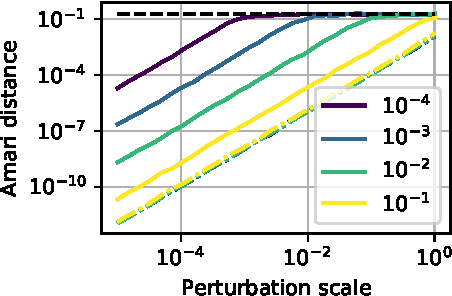
\includegraphics[width=.99\linewidth]{figures/amvica/multicca_gap_jd.pdf}
\caption{Amari distance between true mixing matrices and estimates of Multiset CCA when covariances are perturbed. Different curves correspond to different eigen-gaps. When the gap is small, a small perturbation can lead to complete mixing. Joint-diagonalization (colored dotted lines) fixes the problem.}
\label{fig:cca_gap}
\vspace{-1.5em}
\end{wrapfigure}
We begin with an empirical illustration. We take $m=3$, $p=2$, and $\Sigma_i$ such that $\lambda_1 = 2 + \varepsilon$ and $\lambda_2 =2$ for $\varepsilon > 0$.
%
In this way, we can control the \emph{eigen-gap} of the problem, $\varepsilon$.
%
%
We take $W_i$ the outputs of Multiset CCA applied to the true covariances $C_{ij}$.
%
Then, we generate a perturbation $\Delta = \delta \cdot S$, where $S$ is a random positive symmetric $pm \times pm$ matrix of norm $1$, and $\delta >0$ controls the scale of the perturbation. 
%
We take $\Delta_{ij}$ the $p\times p$ block of $\Delta$ in position $(i, j)$, and $\tilde{W}_i$ the output of Multiset CCA applied to the covariances $C_{ij} + \Delta_{ij}$.
%
We finally compute the sum of the Amari distance between the $W_i$ and $\tilde{W}_i$: the Amari distance measures how close the two matrices are, up to scale and permutation~\cite{amari1996new}.
%\Alex{add ref to paper that explicits the Amari distance}
Fig~\ref{fig:cca_gap} displays the median Amari distance over 100 random repetitions, as the perturbation scale $\delta$ increases. The different curves correspond to different values of the eigen-gap $\varepsilon$. We see clearly that the robustness of Multiset CCA critically depends on the eigen-gap, and when it is small, even a small perturbation of the input (due, for instance, to sampling noise) can lead to large estimation errors.


This problem is very general and well studied~\cite{stewart1973error}: the mapping from matrices to (generalized) eigenvectors is highly non-smooth.
%
However, the gist of our method is that the \emph{span} of the leading $p$ eigenvectors is smooth, as long as there is a large enough gap between  $\lambda_p$ and $\lambda_{p+1}$.
For our specific problem we have the following bounds, derived from Prop.~\ref{prop:eigvals_from_noise}.
\begin{prop}
  We let $\sigma_{\max} = \max_{ij}\Sigma_{ij}$ and $\sigma_{\min} = \min_{ij}\Sigma_{ij}$. Then, $\lambda_p \geq 1 + \frac{m-1}{1+\sigma_{\max}}$, while $\lambda_{p+1}\leq 1 - \frac{1}{1 + \sigma_{min}}$.
\end{prop}
As a consequence, we have $\lambda_{p} -\lambda_{p+1} \geq \frac{m-1}{1+\sigma_{\max}} + \frac{1}{1+ \sigma_{\min}}$: the gap between these eigenvalues increases with $m$, and decreases with the noise power.

  \begin{algorithm}[H]
    \SetAlgoLined
  \caption{ShICA-J}
  \label{algo:shicaj}
  \KwIn{Covariances $\tilde{C}_{ij} =
    \bbE[\xb_i\xb_j^{\top}]$}
    $(\tilde{W}_i)_i \leftarrow \mathrm{MultisetCCA}((\tilde{C}_{ij})_{ij})$ \\
        $Q \leftarrow
        \mathrm{JointDiag}((\tilde{W}_i\tilde{C}_{ii}\tilde{W}_i^{\top})_i)$ \\
       $\Gamma_{ij} \leftarrow Q\tilde{W}_i\tilde{C}_{ij}W_j^\top Q^\top$ \\
       $(\Phi_i)_i \leftarrow \mathrm{Scaling}((\Gamma_{ij})_{ij})$ \\
   \Return{Unmixing matrices $(\Phi_iQ\tilde{W}_i)_i$}
  \end{algorithm}

In this setting, when the magnitude of the perturbation $\Delta$ is smaller than $\lambda_{p}-\lambda_{p+1}$, ~\cite{stewart1973error} indicates that $\mathrm{Span}([W_1, \dots, W_m]^{\top})\simeq \mathrm{Span}([\tilde{W}_1,\dots, \tilde{W}_m]^\top)$, where $[W_1, \dots, W_m]^{\top}\in\bbR^{pm\times p}$ is the vertical concatenation of the $W_i$'s.
In turn, this shows that there exists a matrix $Q\in\bbR^{p\times p}$ such that
%
%
\begin{equation}
    \label{eq:justif_jd}
    W_i \simeq Q\tilde{W}_i\enspace \text{for all} \enspace i.
\end{equation}

We propose to use joint-diagonalization to recover the matrix $Q$. Given the $\tilde{W}_i$'s, we consider the set of symmetric matrices $\tilde{K}_i = \tilde{W}_i\tilde{C}_{ii}\tilde{W}_i^{\top}$, where $\tilde{C}_{ii}$ is the contaminated covariance of $\xb_i$. Following Eq.~\eqref{eq:justif_jd}, we have $Q\tilde{K}_iQ^{\top} = W_i \tilde{C}_{ii}W_i^{\top}$, and using Theorem~\ref{th:eig}, we have $Q\tilde{K}_iQ^{\top} = P\Gamma_i A_i^{-1}\tilde{C}_{ii}A_i^{-\top}\Gamma_iP^{\top}$. Since $\tilde{C}_{ii}$ is close to $C_{ii} = A_i (I_p + \Sigma_i)A_i^\top$, the matrix $P\Gamma_i A_i^{-1}\tilde{C}_{ii}A_i^{-\top}\Gamma_iP^{\top}$ is almost diagonal.
%
In other words, the matrix $Q$ is an approximate diagonalizer of the $\tilde{K}_i$'s, and we approximate $Q$ by joint-diagonalization of the $\tilde{K}_i$'s. In Fig~\ref{fig:cca_gap}, we see that this procedure mitigates the problems of multiset-CCA, and gets uniformly better performance regardless of the eigen-gap.
%
In practice, we use a fast joint-diagonalization algorithm~\cite{ablin2018beyond} to minimize a joint-diagonalization criterion for positive symmetric matrices~\cite{pham2001joint}. The estimated unmixing matrices $U_i = Q\tilde{W}_i$ correspond to the true unmixing matrices only up to some scaling: the information that the components are of unit variance is lost.

\textbf{Scale estimation}
We form the matrices $\Gamma_{ij} = U_i\tilde{C}_{ij}U_j^\top$. In order to estimate the scalings, we solve $
\min_{(\Phi_i)} \sum_{i\neq j} \| \Phi_i \diag(\Gamma_{ij}) \Phi_j - I_p \|_F^2$
where the $\Phi_i$ are diagonal matrices.
This function is readily minimized with respect to one of the $\Phi_i$ by the formula
$\Phi_i = \frac{\sum_{j \neq i} \Phi_j \diag(Y_{ij})}{\sum_{j \neq i} \Phi_j^2 \diag(Y_{ij})^2}$ (derivations in Appendix~\ref{app:fixedpoint}). We then iterate the previous formula over $i$ until convergence.
The final estimates of the unmixing matrices are given by
$(\Phi_i U_i)_{i=1}^m$. The full procedure, called ShICA-J, is summarized in Algorithm~\ref{algo:shicaj}.

\subsection{Estimation of noise covariance and inference of shared components}

In practice, it is important to estimate noise co-variances $\Sigma_i$ in order to take advantage of the fact that some views are noisier than others. As it is well known in classical factor analysis, modelling noise variances allows the model to virtually discard variables, or subjects, that are particularly noisy. 

Using the ShICA model with Gaussian components, we derive noise covariances estimate directly from maximum likelihood. We use an expectation-maximization (EM) algorithm, which is especially fast because noise updates are in closed-form. Following derivations given in appendix~\ref{conditional_density}, the sufficient statistics in the E-step are given by 
\begin{align}
\label{mmse1}
\EE[\sbb|\xb]= \left(\sum_{i=1}^m \Sigma_i^{-1}  + I \right)^{-1}  \sum_{i=1}^m \left(\Sigma_i^{-1} \yb_i \right)
     && \VV[\sbb|\xb]= (\sum_{i=1}^m \Sigma_i^{-1}  + I)^{-1}
\end{align}
Incorporating the M-step we get the following updates that only depend on the covariance matrices:
$
\Sigma_i \leftarrow \diag(\hat{C_{ii}} - 2 \VV[\sbb | \xb]  \sum_{j=1}^m \Sigma_j^{-1} \hat{C}_{ji}  + \VV[\sbb | \xb]  \sum_{j = 1}^m \sum_{l = 1}^m \left(\Sigma_j^{-1} \hat{C}_{jl} \Sigma_l^{-1} \right) \VV[\sbb | \xb] + \VV[\sbb | \xb])
$
%We observe very fast convergence ($10$ iterations are usually enough to reach gradients $\ell_2$ norm below $10^{-4}$).

\section{ShICA-ML: Maximum likelihood for non-Gaussian components}
ShICA-J only uses second order statistics. However, the ShICA model~\eqref{eq:model} allows for non-Gaussian components. We now propose an algorithm for fitting the ShICA model that assumes non-Gaussian components so that it can separate Gaussian and non-Gaussian components.
%\aapo{[Aapo: Motivate and link to previous sections]}
We estimate the parameters by maximum likelihood. Since most non-Gaussian components in real data are super-Gaussian, we assume that the non-Gaussian components $\sbb$ have the super-Gaussian density \\ $p(s_j) = \frac12\left(\mathcal{N}( s_j; 0, \frac12) + \mathcal{N}( s_j; 0, \frac{3}{2})\right) \enspace.$

We propose to maximize the log-likelihood using a generalized
EM~\cite{neal1998view, dempster1977maximum}. Derivations are available in Appendix~\ref{app:emestep}. Like in the previous section, the E-step is in closed-form yielding the following sufficient statistics:
\begin{align}
\label{mmse2}
\EE[\sbb | \xb] = \frac{\sum_{\alpha \in \{\frac12, \frac32
    \}}\theta_{\alpha} \eb_{\alpha}}{\sum_{\alpha \in
    \{\frac12, \frac32 \}}\theta_{\alpha}}
    && 
    \VV[\sbb | \xb] = \frac{\sum_{\alpha \in \{\frac12, \frac32
    \}}\theta_{\alpha} V_{\alpha}}{\sum_{\alpha \in
    \{\frac12, \frac32 \}}\theta_{\alpha}} 
\end{align}
    where
    $\eb_{\alpha}= \left(\sum_{i=1}^m \Sigma_i^{-1}  + \frac1{\alpha}I \right)^{-1}  \sum_{i=1}^m \left(\Sigma_i^{-1} \yb_i \right)$,  $V_{\alpha} = (\sum_{i=1}^m \Sigma_i^{-1}  + \frac1{\alpha}I)^{-1}$ and $\theta_{\alpha} = \mathcal{N}((\sum_{i=1}^m \Sigma_i^{-1})^{-1} \Sigma_i^{-1} \yb_i; 0, \alpha I + (\sum_{i=1}^m \Sigma_i^{-1})^{-1})$ with $\yb_i = W_i \xb_i$.
Noise updates are in closed-form and given by:
$\Sigma_i \leftarrow  \diag((\yb_i - \EE[\sbb | \xb]) (\yb_i - \EE[\sbb | \xb])^{\top}+ \VV[\sbb | \xb])$.
However, no closed-form is available for the updates of unmixing matrices. We therefore perform quasi-Newton updates given by
$W_i \leftarrow (I - \rho (\widehat{\mathcal{H}^{W_i}})^{-1} \mathcal{G}^{W_i}) W_i$ where $\rho \in \mathbb{R}$ is chosen by backtracking line-search, 
$\widehat{\mathcal{H}^{W_i}_{a, b, c, d}} =  \delta_{ad} \delta_{bc} + \delta_{ac} \delta_{bd}\frac{(y_{ib})^2}{\Sigma_{ia}}$ is an approximation of the Hessian of the negative complete log-likelihood and $\mathcal{G}^{W_i} = -I + (\Sigma_i)^{-1}(\yb_i - \mathbb{E}[\sbb|\xb])(\yb_i)^{\top}$ is the gradient.

We alternate between computing the statistics $\mathbb{E}[\sbb|\xb]$, 
$\mathbb{V}[\sbb|\xb]$ (E-step) and updates of parameters $\Sigma_i$ and $W_i$ for $i=1 \dots m$ (M-step). Let us highlight that our EM algorithm and in particular the E-step resembles the one used in~\cite{moulines1997maximum}. However because they assume noise on the sensors and not on the components, their formula for $\EE[\sbb| \xb]$ involves a sum with $2^p$ terms whereas we have only $2$ terms. The resulting method is called ShICA-ML.

\paragraph{Minimum mean square error estimates in ShICA}
In ShICA-J as well as in ShICA-ML, we have a closed-form for the expected components given the data $\EE[\sbb | \xb]$, shown in equation~\eqref{mmse1} and~\eqref{mmse2} respectively. This provides minimum mean square error estimates of the shared components, and is an important benefit of explicitly modelling shared components in a probabilistic framework.
%\aapo{[Aapo: The formulas for Es|x should be given as numbered equations, and they should be referred to here. But this is too short to be a proper section...]}

% \section{An alternate quasi-newton algorithm for MIFA}


% We estimate the parameters of model~\eqref{model} ($W_i$ and $\Sigma_i$) via maximum likelihood.
% As shown in Appendix~\ref{likelihood_derivation}, the negative log-likelihood is given by
% \begin{align}
%   \mathcal{L} = &\sum_{i=1}^m\left(-\log|W_i| + \frac12 \log |\Sigma_i|\right) + \frac12 \log(|\sum_{i=1}^m \Sigma_i^{-1} + I|) + \frac12 (\sum_{i=1}^m \langle \yb_i | \Sigma_i^{-1} \yb_i \rangle \\&  - \frac12 \langle \left(\sum_{i=1}^m \Sigma_i^{-1} + I \right)^{-1} \sum_{i=1}^m \left(\Sigma_i^{-1} \yb_i \right) | \sum_{i=1}^m \left(\Sigma_i^{-1} \yb_i \right) \rangle)
% \end{align}

% We optimize this likelihood using expectation-maximization (EM)~\addref.

% The completed likelihood is given by
% \begin{equation}
%   p(\xb, \sbb) = p(\xb_i | \sbb) p(\sbb)=  |W_i| \Ncal(\yb_i; \sbb, \Sigma_i) \Ncal(\sbb; 0, I_k)
% \end{equation}
% Therefore the negative completed log-likelihood is a quadratic function of the
% components so only second moments of $\sbb | \xb$ are needed. It turns out that we
% can compute $\sbb | \xb$ exactly. Derivations given in appendix~\ref{conditional_density} yield:
% \begin{align}
%   &\sbb|\xb \sim \Ncal( \EE[\sbb|\xb], \VV[\sbb | \xb]) \\
%   & \text{where } \enspace \EE[\sbb|\xb]= \left(\sum_{i=1}^m \Sigma_i^{-1}  + I \right)^{-1}  \sum_{i=1}^m \left(\Sigma_i^{-1} \yb_i \right) \text{ and } \VV[\sbb|\xb]= (\sum_{i=1}^m \Sigma_i^{-1}  + I)^{-1}
% \end{align}

% The function to minimize in the M-step is therefore given by:
% \begin{align}
%   \Jcal = \sum_{i=1}^m -\log(|W_i|) +\log(|\Sigma_i|) + \frac12 \tr(\Sigma_i^{-1} \left[(\yb_i - \EE[\sbb | \xb]) (\yb_i - \EE[\sbb | \xb])^{\top}+ \VV[\sbb | \xb]\right])  
% \end{align}

% We get closed-form updates for $\Sigma_i$ given by
% \[
% \Sigma_i \leftarrow  \diag((\yb_i - \EE[\sbb | \xb]) (\yb_i - \EE[\sbb | \xb])^{\top}+ \VV[\sbb | \xb])
% \]
% Updates with respect to $W_i$ are obtained through a quasi-newton step:
% $W_i \leftarrow (I - \rho H_i G_i^{-1}) W_i$ where the relative gradient is
% given by
% $G_i = I - \Sigma_i^{-1}(\yb_i - \EE[\sbb | \xb])\yb_i^{\top}$ and while the
% true Hessian is given by $H_{i, abcd} = \delta_{a,c} \frac{y_{i, b} y_{i,
%     d}}{\Sigma_{i, a}}$, we use for increased speed, the following
% approximation: $\tilde{H}_{i, abcd} = \delta_{a, c} \delta_{b,d}
% \frac{y_{i, b}^2}{\Sigma_{i, a}}$ which is exact when the unmixed
% data are truly independent. The step-size $\rho$ is chosen by backtracking
% line-search.

% Note that the likelihood and therefore the updates only depend on the covariance
% of the data. Therefore in practice, we pre-compute the covariances $\xb_i \xb_j^{\top}$ for
% all $1 \leq i \leq m$ and $1 \leq i \leq m$ and do not use the original data
% anymore. This provide a great speed-up when the number of samples is high.


% \begin{ack}
% Use unnumbered first level headings for the acknowledgments. All acknowledgments
% go at the end of the paper before the list of references. Moreover, you are required to declare
% funding (financial activities supporting the submitted work) and competing interests (related financial activities outside the submitted work).
% More information about this disclosure can be found at: \url{https://neurips.cc/Conferences/2021/PaperInformation/FundingDisclosure}.

% Do {\bf not} include this section in the anonymized submission, only in the final paper. You can use the \texttt{ack} environment provided in the style file to autmoatically hide this section in the anonymized submission.
% \end{ack}

% \section{A generalized eigenvalue approach for MIFA}
% While maximum-likelihood approaches possess several important statistical properties that make them attractive, a major drawback is the slowness of the algorithms. 

% These method also require the likelihood to be well defined, and prevents dimension reduction without a more complicated model: for the likelihood to be well defined, we must assume that $A_i$ is square, invertible.

% If we only consider two views, the model of MIFA in equation~\eqref{model} is
% the model of probabilistic CCA~\addref but with a different noise covariance.
% Many multiview CCA methods exists~\addref. They are typically referred to as
% Multiset CCA and differ by the objective they optimize as well as the
% constraints they put on the canonical vectors~\addref. A tractable formulation is given
% by the SUMCOR~\addref objective:
% \begin{align}
%   \rho(\vb_1 \dots \vb_m) = \sum_{i=1}^m \sum_{j \neq i}^m \vb_i^{\top} C_{ij} \vb_j,  \text{ such that } \forall i, \sum_{i=1}^m\vb_i^{\top} C_{ii} \vb_i = 1
% \end{align}
% which we can write in matrix form as
% \begin{align}
%   \rho(V_1 \dots V_m) = \sum_{i=1}^m \sum_{j \neq i}^m \tr(V_i^{\top} C_{ij} V_j),  \text{ such that } \forall i, \sum_{i=1}^m V_i^{\top} C_{ii} V_i = I
% \end{align}
% for $V^i \in \mathbb{R}^{k, p}$.

% The first order conditions yield the following generalized eigenvalue problem
% \begin{align}
%   \begin{bmatrix} C_{11} & \dots & C_{1m} \\
%     \vdots & \ddots & \vdots  \\
%     C_{m1} & \dots  &C_{mm}
%   \end{bmatrix} \begin{bmatrix} V_1 \\ \vdots \\ V_m \end{bmatrix} = \begin{bmatrix} C_{11} &  & 0 \\
%      & \ddots &   \\
%     0 &   &C_{mm}
%   \end{bmatrix} \begin{bmatrix} V_1 \\ \vdots \\ V_m \end{bmatrix} \Lambda  \label{problem}
% \end{align}
% where $\Lambda \in \mathbb{R}^{kxk}$ is a matrix of Lagrange
% multipliers. The $k$ eigenvectors corresponding to the largest eigenvalues yield
% the solution up to a global rotation.

% The following lemma shows that minimizing the above objective leads to estimates
% of the true unmixing matrices up to a view specific scaling and a global rotation.
% \begin{prop}
%   \label{gev}
%   Assume that data are generated from model~\eqref{model} with mixing matrix
%   $A_i \in \mathbb{R}^{k \times k}$ and assume all subjects have distinct
%   noise covariances $\Sigma_i$. Then, in the limit of large samples $n=\infty$,
%   the $k$ first eigenvectors of the
%   generalized eigenvalue problem~\eqref{problem} are given by
%   $\begin{bmatrix} W_1^{\top} \Gamma_1 P \\ \vdots \\ W_m^{\top} \Gamma_m P \end{bmatrix}$ where
%   $\Gamma_i$ are scale matrices and $P$ is a permutation matrix.
% \end{prop}


% \begin{prop}
%   \label{finite}
%   Assume $n < \infty$ samples are generated from model~\eqref{model} with mixing matrix
%   $A_i \in \mathbb{R}^{k \times k}$ and assume all subjects have distinct
%   noise covariances $\Sigma_i$. Then, assuming the empirical covariance is close to
%   the actual covariance the $k$ first eigenvectors are given by the formula of
%   prop~\label{gev} up to a global rotation.
% \end{prop}

  

% \section{Related Work}
% ShICA combines theory and methods coming from different branches of ``component analysis''. It can be viewed as a GroupICA method, as an extension of Multiset CCA, as an Independent Vector Analysis method or, crucially, as an extension of the shared response model. In the setting studied here, ShICA improves upon all existing methods.

% \paragraph{GroupICA}
% GroupICA methods extract independent components from multiple datasets. In its original form\cite{calhoun2001method}, views are concatenated and then a PCA is applied yielding reduced data on which ICA is applied. One can also reduce the data using Multiset CCA instead of PCA, giving a method called \emph{CanICA}~\cite{varoquaux2009canica}. Other works~\cite{Esposito05NI, Hyva11NI} apply ICA separately on the datasets and attempt to match the decompositions afterwards.
% Although these works provide very fast methods, they do not rely on a well defined model like ShICA. %In contrast, the procedure in ShICA-J is based on an explicit model.
% Other GroupICA methods impose some structure on the mixing matrices such as the tensorial method of~\cite{beckmann2005tensorial} or the group tensor model in~\cite{guo2008unified} (which assumes identical mixing matrices up to a scaling) or \cite{svensen2002ica} (which assumes identical mixing matrices but different components). In ShICA the mixing matrices are only constrained to be invertible.
% Lastly, maximum-likelihood based methods exist such as \emph{MultiViewICA}~\cite{richard2020modeling} or the full model of~\cite{guo2008unified}. These methods are weaker than ShICA as they assume non-Gaussianity, the same noise covariance across views and lack a principled method for shared response inference.
% %\aapo{These methods are weaker than from ShICA as they assume non-Gaussianity, the same noise covariance across views, and lack a principles method for shared response inference. [I hope this is all correct? - Hugo:We have seen that multiview ICA can separate Gaussian components but in practice it does it quite poorly. However we could have derived a principle method for shared response inference (but that cannot take into account the fact the some views are noisier than others) ]}
% %Aapo: But our comparison here should be limited to what is actually done and said in the papers, not what the methods could be able to do with further development. Hugo: Ok agreed !

% \paragraph{Multiset CCA}
% In its basic formulation, CCA identifies a shared space between two datasets.
% The extension to more than two datasets is ambiguous, and many
% different generalized CCA methods have been proposed. \cite{kettenring1971canonical} introduces 6 objective functions that reduce to CCA when $m=2$ and \cite{nielsen2002multiset} considered 4 different possible constrains leading to 24 different formulations of Multiset CCA. The formulation used in ShICA-J is refered to in~\cite{nielsen2002multiset} as SUMCORR with constraint 4 which is one of the fastest as it reduces to solving a generalized eigenvalue problem. The fact that CCA solves a well defined probabilistic model has first been studied in~\cite{bach2005probabilistic} where it is shown that CCA is identical to multiple battery factor analysis~\cite{browne1980factor} (restricted to 2 views). This latter formulation differs from our model in that the noise is added on the sensors and not on the components which makes the model unidentifiable. Identifiable variants and
% generalizations can be obtained by imposing sparsity on the mixing matrices such as in~\cite{archambeau2008sparse, klami2014group, witten2009extensions} or non-negativity~\cite{DELEUS2011143}.
% The work in~\cite{li2009joint} exhibits a set of sufficient (but not necessary) conditions under which a well defined model can be learnt by the formulation of Multiset CCA used in ShICA-J. The set of conditions we exhibit in this work are necessary and sufficient. We further emphasize that basic Multiset CCA provides a poor estimator as explained in Section~\ref{sec:samplingnoise}.

% \paragraph{Independent vector analysis}
% Independent vector analysis~\cite{lee2008independent} (IVA) models the data as a linear mixture of independent components $\xb_i = A_i \sbb_i$ where each component $s_{ij}$ of a given view $i$ can depend on the corresponding component in other views ($(s_{ij})_{i=1}^m$ are not independent).
% % the components $\sbb_i \in \bbR^{p}$ differ across subjects but component $j$  \bt{the joint distribution of s samples ? it is unclear what j stands for} is not independent across subjects
% Practical implementations of this very general idea assume a distribution for $p((s_{ij})_{i=1}^m)$. In IVA-L~\cite{lee2008independent}, $p((s_{ij})_{i=1}^m) \propto \exp(-\sqrt{\sum_i (s_{ij})^2})$ (so the variance of each component in each view is assumed to be the same), in IVA-G~\cite{anderson2011joint} or in~\cite{via2011maximum}, $p((s_{ij})_{i=1}^m) \sim \mathcal{N}(0, R_{ss})$ and~\cite{engberg2016independent} proposed a normal inverse-Gamma density. The model of ShICA can be seen as an instance of IVA %(where $p$ in ShICA-ML is a Gaussian mixture in which variances are learnt), 
% which specifically enables extraction of shared components from the subject specific components, unlike previous versions of IVA. In fact, ShICA comes with minimum mean square error estimates for the shared components
% %(given by $\bbE[\sbb | \xb]$) 
% that is often the quantity of interest. By contrast, the model in IVA-L has components that are uncorrelated over views, which is quite unrealistic for fMRI or any MEG/EEG evoked response, while our model is explicitly constructed to be realistic for brain imaging applications.
% The IVA theory provides global identifiability conditions in the Gaussian case (IVA-G)~\cite{via2011joint} and local identifiability conditions in the general case~\cite{anderson2014independent} from which local identifiability conditions of ShICA could be derived. However, in this work, we provide global identifiability conditions for ShICA.
% Lastly, IVA can be performed using joint diagonalization of cross covariances~\cite{li2011joint, congedo2012orthogonal} although multiple matrices have to be learnt and cross-covariances are not necessarily symmetric positive definite which makes the algorithm slower and less principled.

% \paragraph{Shared response model}
% ShICA extracts shared components from multiple datasets, which is also the goal of the shared response model (SRM)~\cite{chen2015reduced}. The robust SRM~\cite{turek2018capturing} also allows to capture subject specific noise. However these models impose orthogonality constraints on the mixing matrices while ShICA does not. Deep variants of SRM exist such as~\cite{chen2016convolutional} but while they release the orthogonality constrain, they are much more computationally demanding. ShICA leverages ICA theory to provide a much more powerful model of shared responses.

% \paragraph{Limitations}
% The main limitation of this work is that the model does not reduce the dimension inside each view. In line with other methods, such view-specific  dimension reduction has to be done by some external method, typically view-specific PCA. Using specialized methods for the estimation of covariances should also be of interest for ShICA-J, where it only relies on sample covariances. Finally, ShICA-ML uses a simple model of a super-Gaussian distribution, while modelling the non-gaussianities in more detail in ShICA-ML should improve the performance.